%%%%%%%%%%%%%%%%%%%%%%%%%%%%%%%%%%%%%%%%%%%%%%%%%%%%%%%%%%%%%%%%%%%%%%%%
% Introduction
%%%%%%%%%%%%%%%%%%%%%%%%%%%%%%%%%%%%%%%%%%%%%%%%%%%%%%%%%%%%%%%%%%%%%%%%
\section{Introduction}
\label{sec:intro}

%\todo[inline]{Manu: use "summary sentences" for paragraphs}
%\todo[inline]{REVIEWER: the theoretical foundations of data cleaning with MLNs should be developed, explained, and discussed in more detail.}

%What is the problem?
% see here for description why data quality is important.
% http://books.google.de/books?hl=en&lr=&id=SULMBFgtwQoC&oi=fnd&pg=PA1&ots=uaNGyVfL7V&sig=RER31QotCCRJeaQq8OafAtpgK1k#v=onepage&q&f=false

Having access to high quality data is of great importance in data analysis. However, in the real world, data is often considered \textit{dirty}, meaning that it contains inaccurate, incomplete, inconsistent, duplicated, or stale values ~\cite{chu2004blissful}. A number of distinct data quality issues are known in the field of Data Quality Management such as \textit{data consistency}, \textit{currency}, \textit{accuracy}, \textit{deduplication} and \textit{information completeness}~\cite{fan2012foundations}. As previous work has observed, such data quality issues may be detrimental to data analysis~\cite{national2013Frontiers,Fan:2008:CFD:1366102.1366103} and cause huge costs to businesses ~\cite{waynew.eckerson2002}. Therefore, improving data quality with respect to business and integrity constraints is a crucial component of data management. 
A common approach to increasing data quality is to formulate a set of \textit{data cleaning rules} that detect semantic errors by utilizing data dependencies~\cite{fan2012foundations, Arasu:2009:LDC:1546683.1547340, Dallachiesa:2013:NCD:2463676.2465327, llunaticVDLB2013b}. However, previous research identified a number of challenges associated with creating such rule sets: 
\todo[inline]{Desiderata: 1.Usability and domain knowledge integration (aka human interaction); 2.Interleaved rules; 3.Automation}
\todo[inline]{Challenges: 1. Various languages and approaches exist but there is a need for expressivity and customization of the rules. Also suitable for non-experts; 2.Holistic treatment of rules and the ability to integrate the “soft” and “hard” rules. 3.The difficulty to find the optimal order of the rules execution}
Firstly, while each such rule may address one data quality issue individually, previous work in~\cite{fan2012foundations} and \cite{Fan:2014:IRM:2628135.2567657} has observed that such rules may \textit{interact}. For instance, a rule that deletes duplicates might perform better if missing data has already been imputed, while, on the other hand, a rule that imputes missing data might perform better if duplicates have already been removed. This means that data quality rules such as deduplication and missing value imputation should be modeled jointly, rather than as separate processes.
Secondly, rules in such a rule-set may need to be \textit{"soft"} and \textit{"hard"} in order to balance constraints of different importance, especially within a set of interacting rules. This makes the creation of such rule sets challenging from a modeling perspective. Defining probabilistic data quality rules enables us to use statistical inference in order to predict errors. 

\todo[inline]{Our hypothesis: While authomatic data cleaning, it is impossible to specify the optimal order of rules execution \cite{Dallachiesa:2013:NCD:2463676.2465327}, therefore we use joint inference for the simultaneous rules execution.}

In this paper, we present an approach to data cleaning based on Statistical Relational Learning (SRL)~\cite{getoor2007introduction} and probabilistic inference. SRL is a branch of machine learning that models joint distributions over relational data. Generally, data quality rules represent relationships between attributes in the database schema. These rules are mainly based on integrity constraints such as functional dependencies~\cite{AbiteboulHV95} on top of a database schema. We show how such functional dependencies, expressed as first-order logic formulas, can be translated into probabilistic-logical languages, allowing us to reason over inconsistencies, duplicates or missing values in a probabilistic way.

\todo[inline]{Contributions: 1.[Frontend] We demonstrate how data cleaning rules based on integrity constraints are modeled within the probabilistic-logic framework such as Markov logic; 2.[Backend/Compiler] We demonstrate how data cleaning problem is expressed as probabilistic graphical model and using joint inference for data correction prediction; 3. [Execution Engine] We demonstrate the empirical study of modeling and errors prediction in the data cleaning by using Markov Logic}
\todo[inline]{Experimental results: Preview.}
 
 \begin{figure}[t]
 \centering
 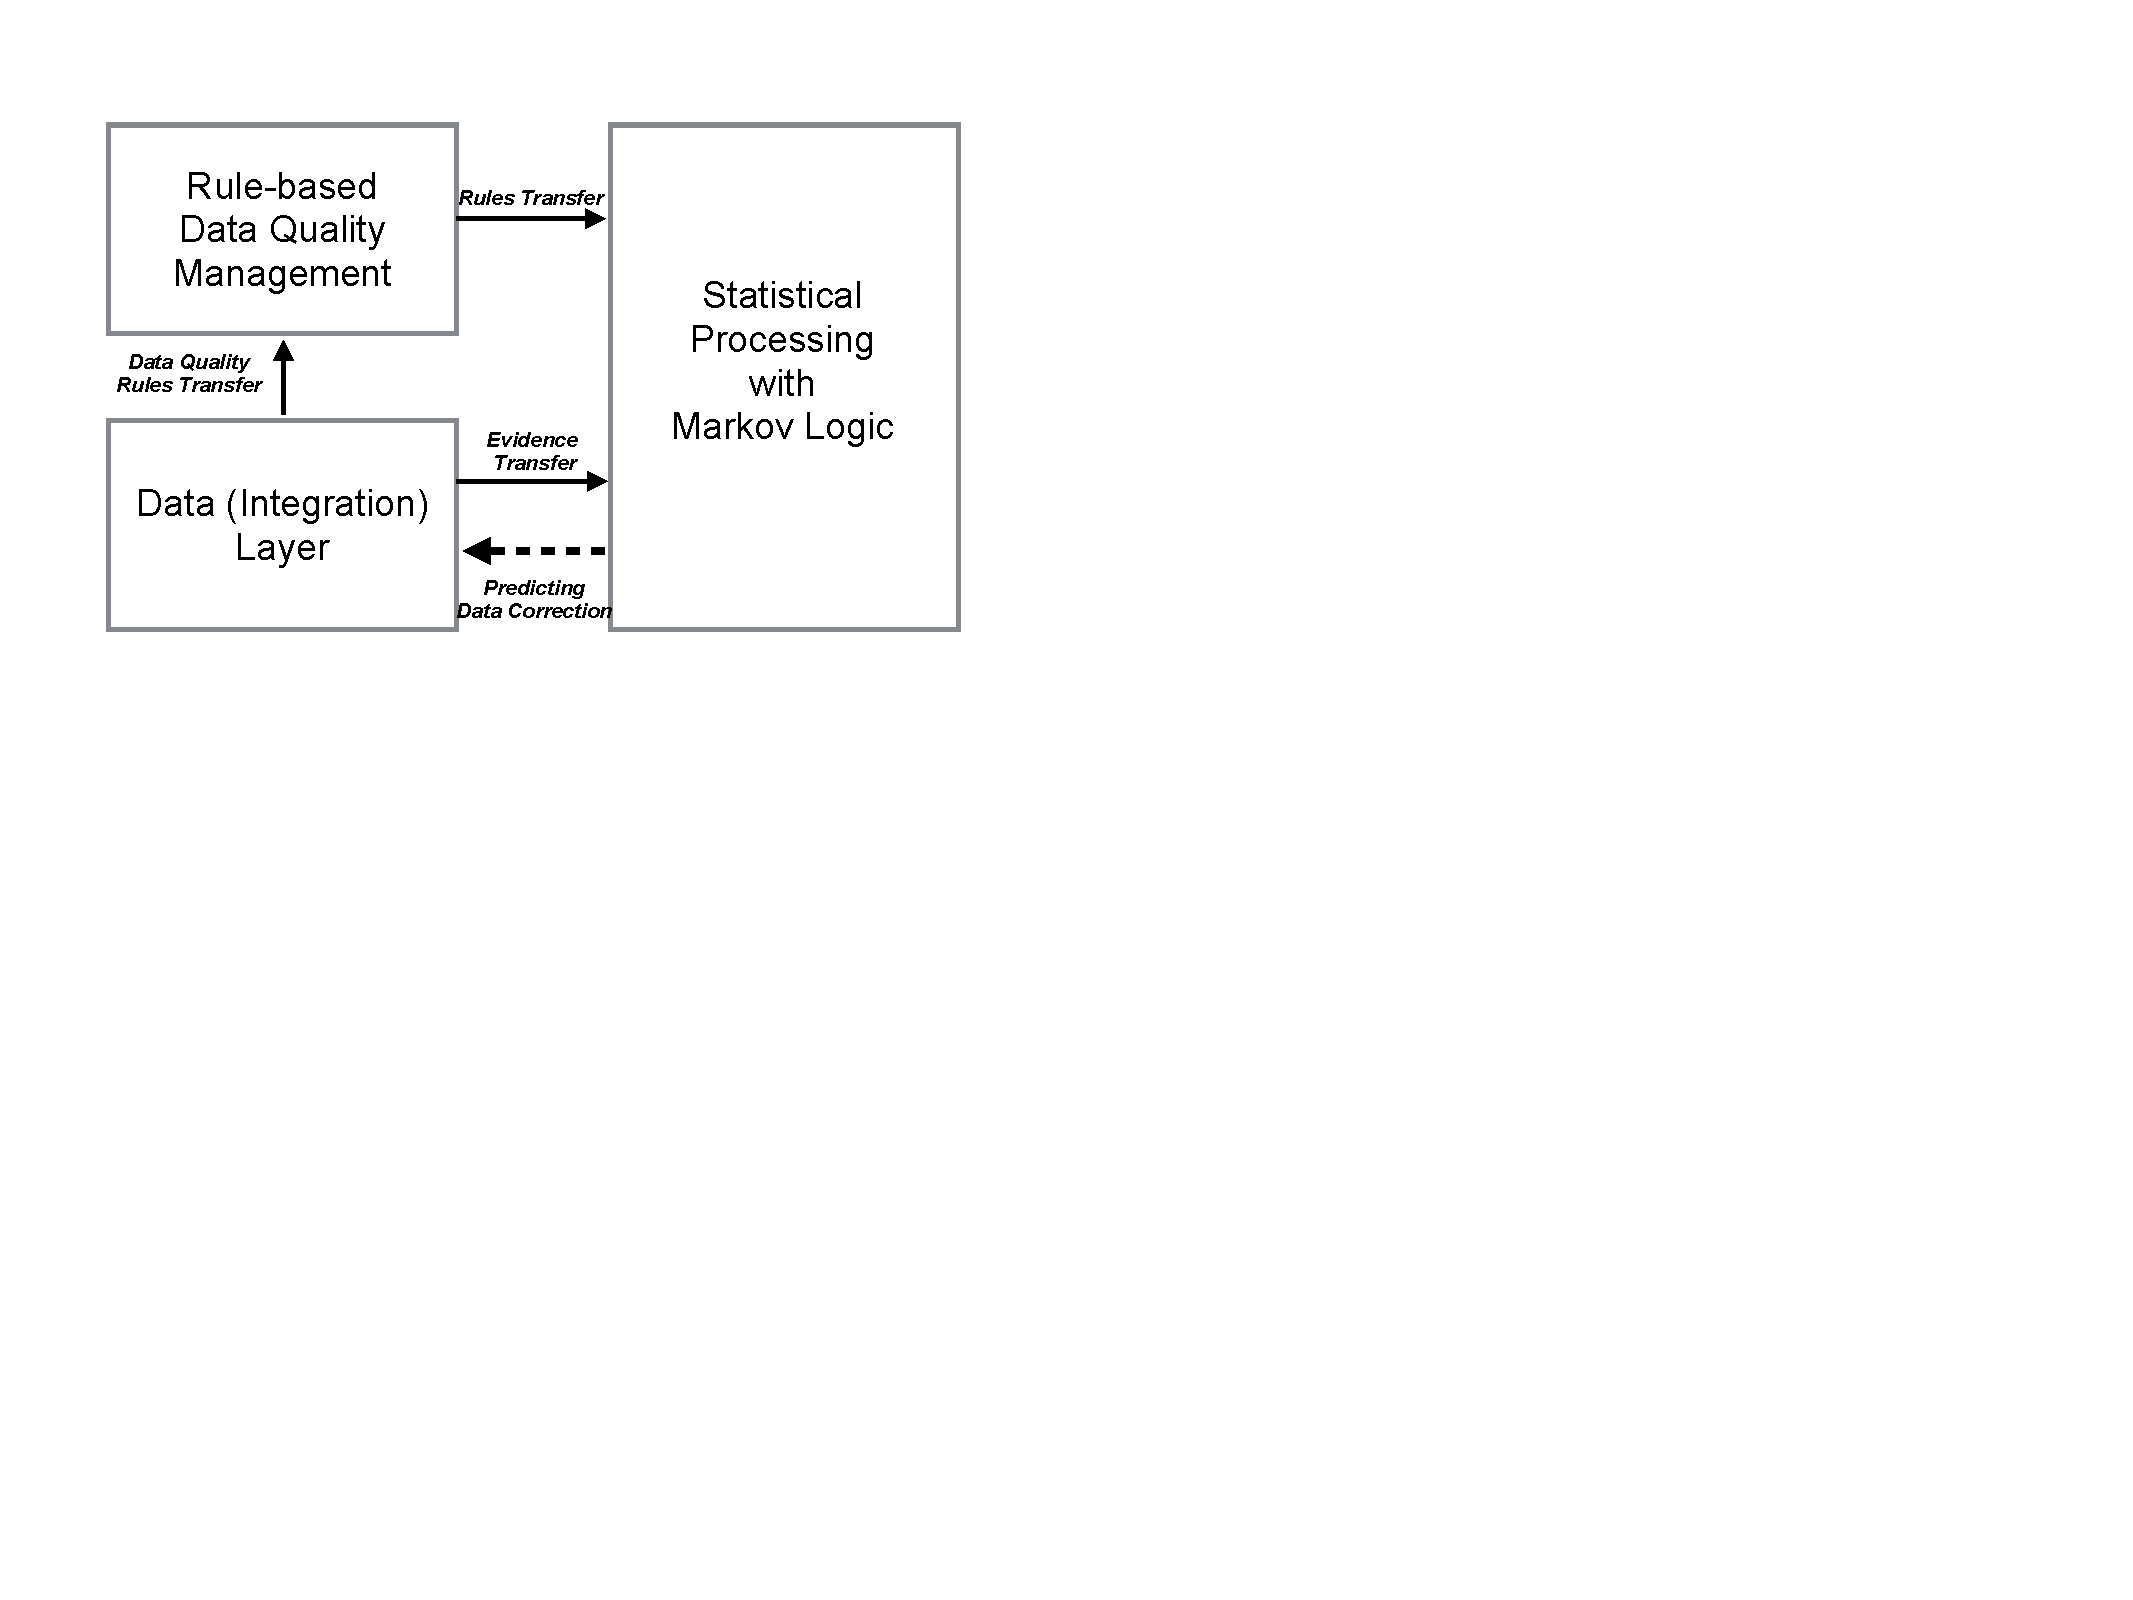
\includegraphics[width=200px, height=140px]{img/system.pdf}
 \caption{Our proposed method for data cleaning based on Markov logic consists of three main components: 
 (I) A \textbf{Rule-based Data Quality Management} component that is based on the data quality rules to address different data quality issues;
 (II) A \textbf{relation prediction} component based on probabilistic inference performed by the Markov logic framework and (III) 
 a \textbf{Data Layer} that includes a number of data sources including relational and semi-structured data.}
 \label{fig:system}
\end{figure}     
